\section{Approach}
\label{sec:approach}

\begin{figure}[th!]
	\centering
	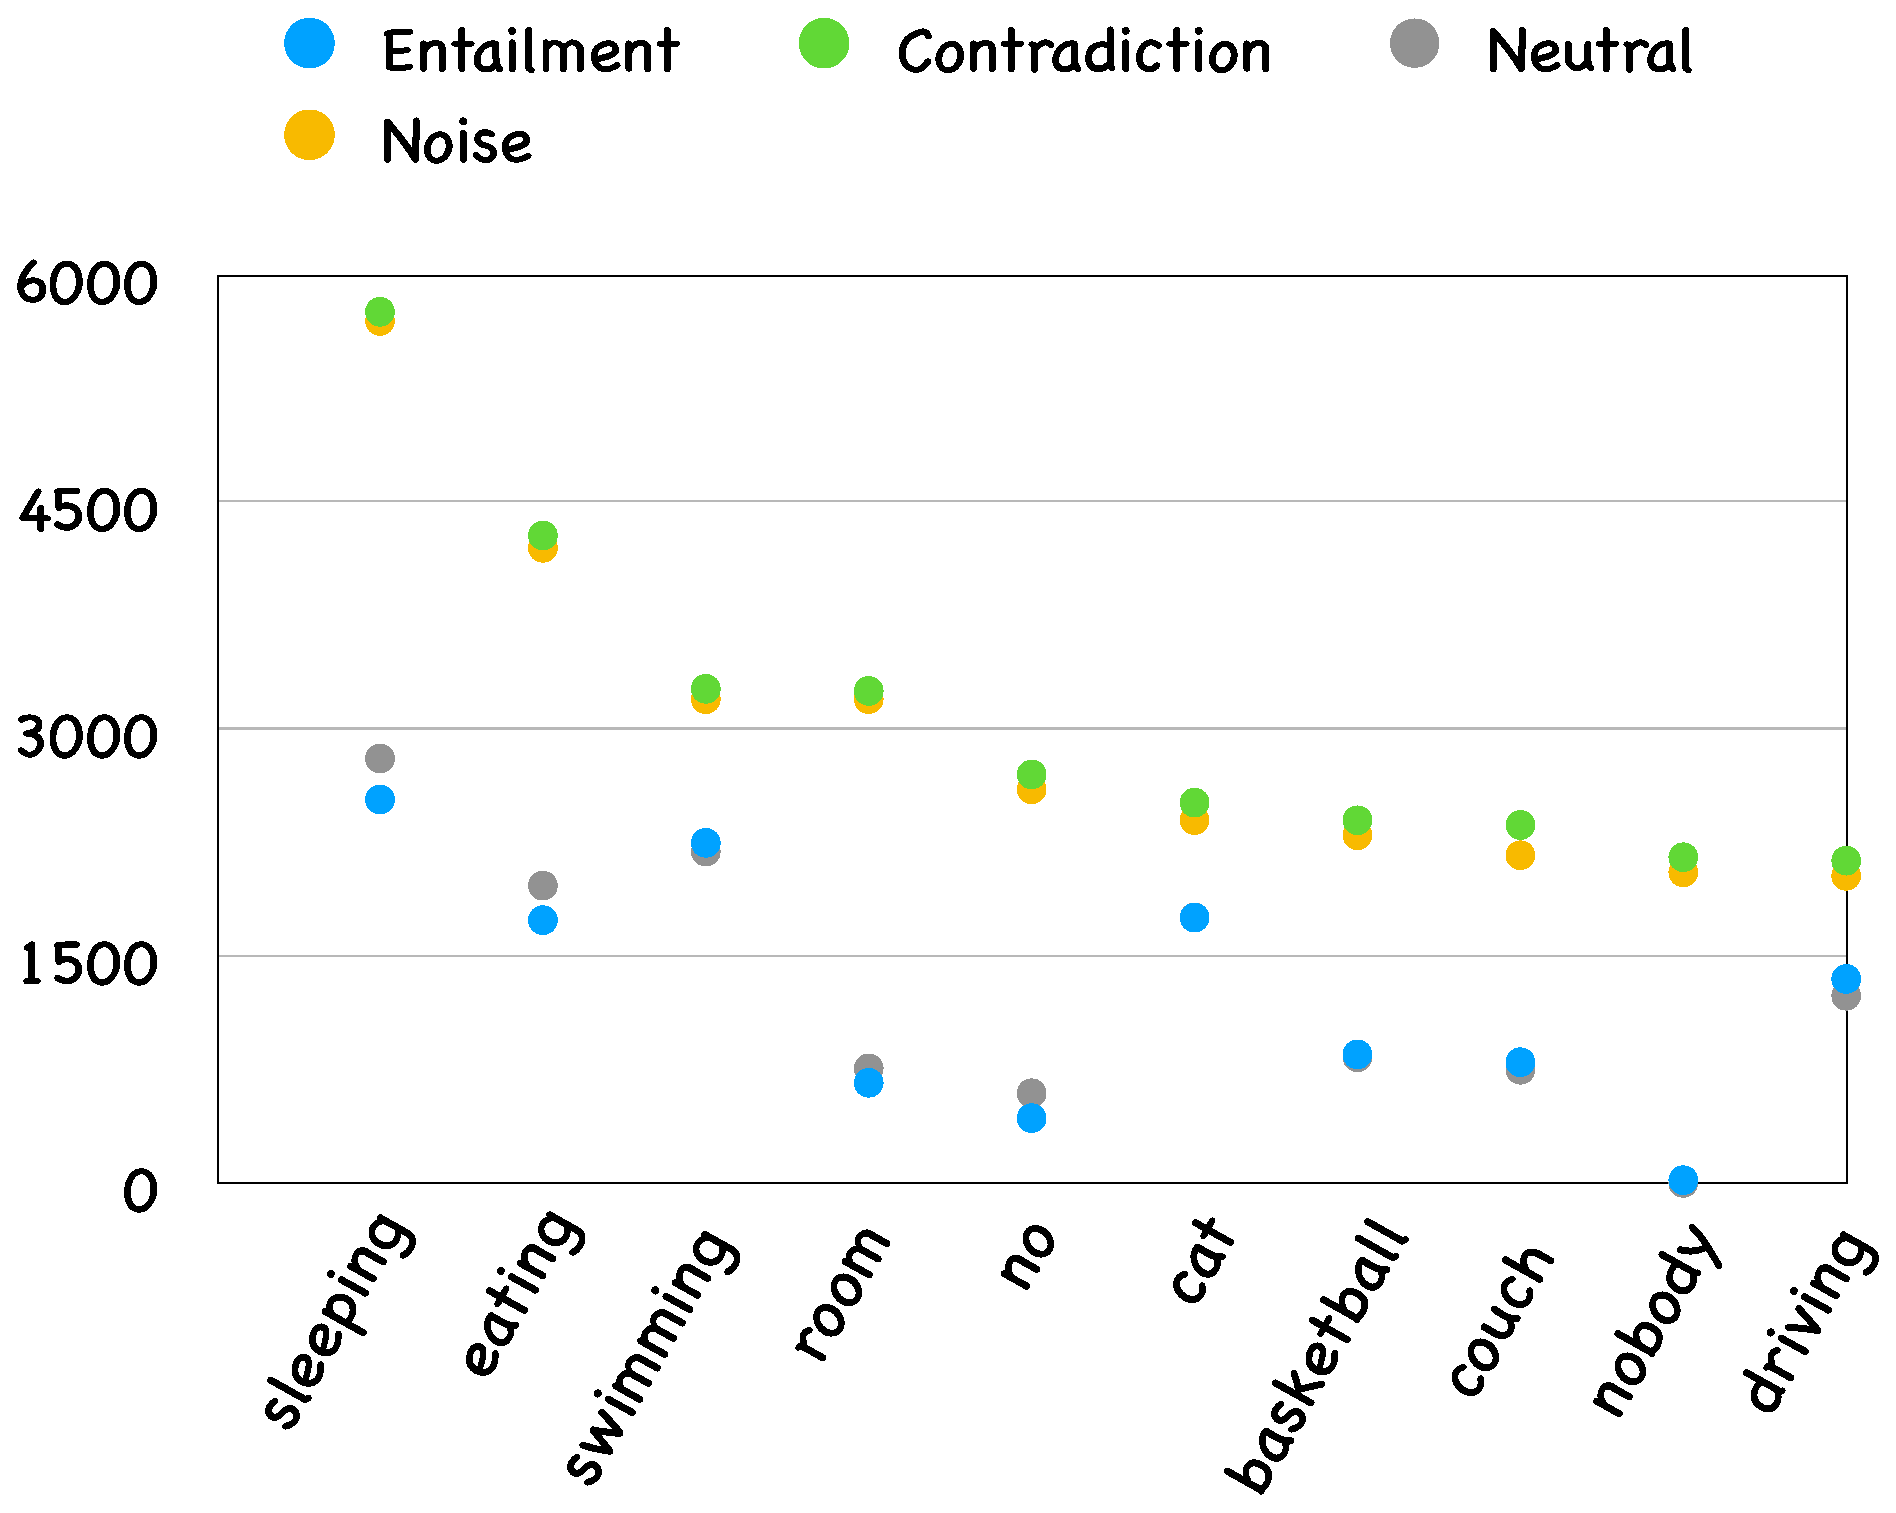
\includegraphics[width=0.4\columnwidth]{figures/noise_balance.eps}
	\caption{The left shows some words we sample from SNLI which mostly appears in Contradiction labeled instances. The right is the new dataset word distribution after we add Noise labeled instances.}
\label{fig:noise_balance}
\end{figure}

\begin{figure}[th!]
	\centering
	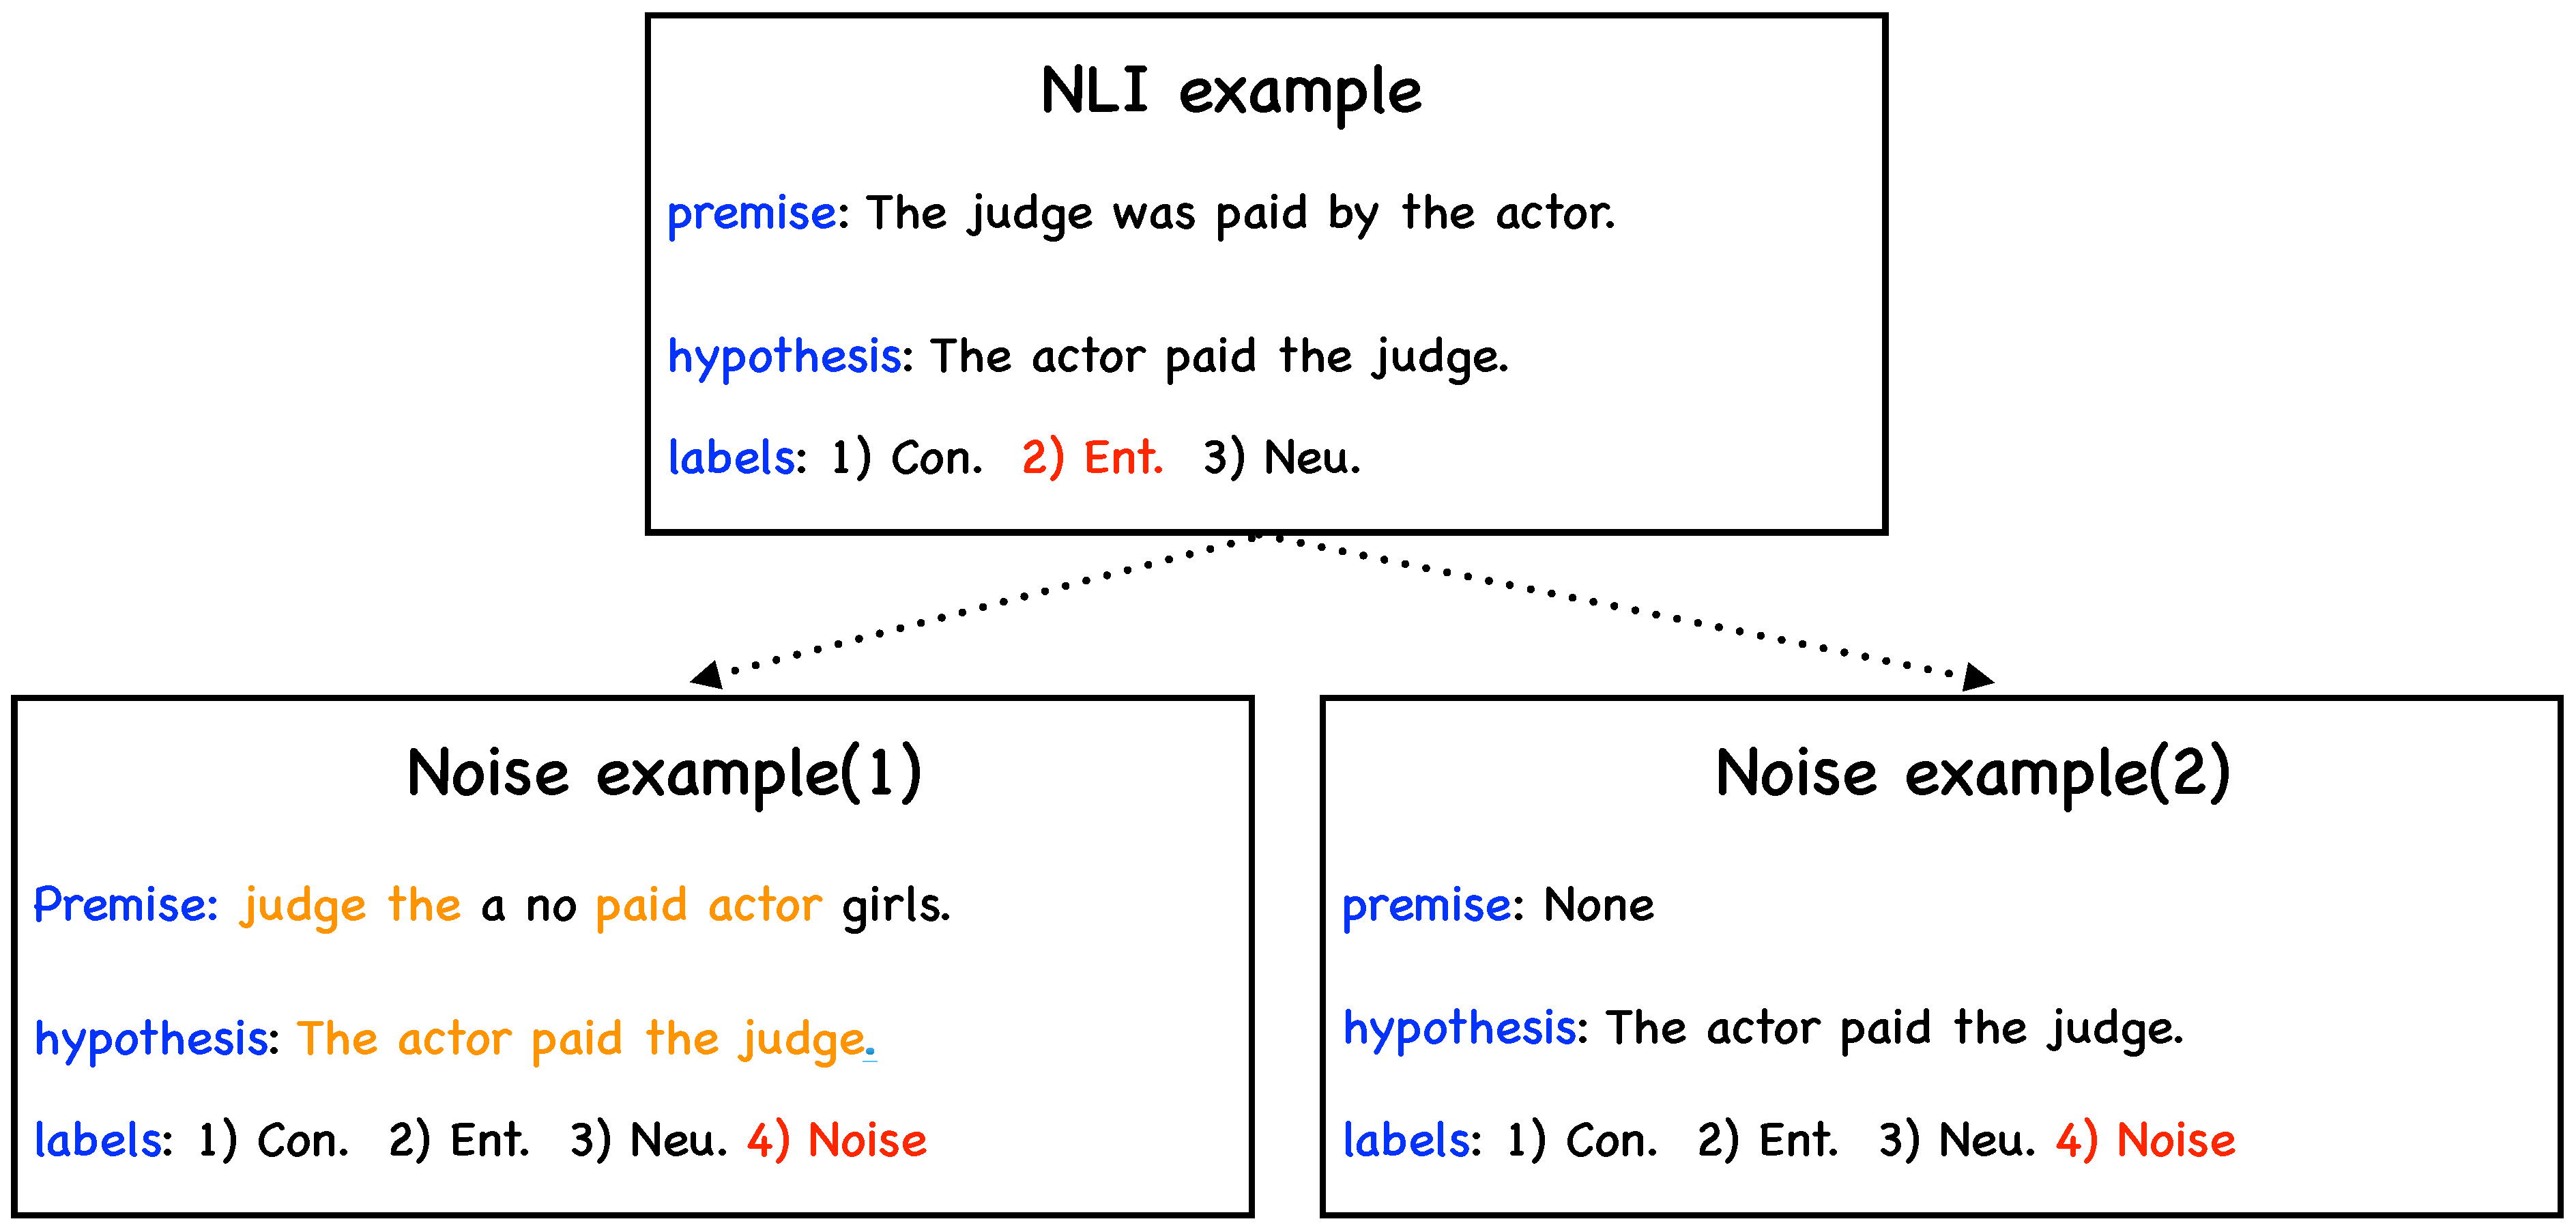
\includegraphics[width=0.8\columnwidth]{figures/noise.eps}
	\caption{We sample some tokens from SNLI and calculate the frequency of each token based on different labels.}
\label{fig:noise2and3}
\end{figure}

In this section, we first formalize the commonsense reasoning classification problem
 and then introduce our three noise data augmentation methods.
 
\subsection{Problem Statement}
\label{sec:problem_statement}
Given a natural language
premise $p$ and a hypothesis $h$, we should judge the 
relation  from the alternative label set $L$ between $p$ and $h$. 
In FEVER, \textit{evidence} corresponds to premise and \textit{claim} 
is hypothesis based on \textit{evidence}. For the shallow spurious features, like 
unbalanced word distribution, word overlap and hypothesis-only, misleading models to
learn reasoning unrelated features and affecting models' robustness, 
our goal is to generate noisy data to weaken these features and improve 
the reasoning ability of models.

\subsection{Noise Data Augmentation Methods}
\label{sec:noise_methods}

\subsubsection{Balanced Distribution Noise}:


As shown in~\figref{fig:noise_balance}, we calculate the frequency of 
each token based on different labels and observe disparities in distribution. 
We show some words which always appears in ``Contradiction'' of SNLI, 
for example, word ``nobody'' almost never appears 
in ``Entailment'' and ``Neutral'' instances which may misguide models to choose 
``Contradiction'' once they find ``nobody'' in an instance. And many nouns like ``cat'' and ``couch'' 
are also highly unbalance. To remedy this issue, we propose to 
make the distribution of each word $w$ in vocabulary set $V$ of the dataset more balance by adding 
new instances with label ``Noise''. The frequency of word $w$ based on label $l_{i}\in{L}$ is denoted as $freq(w, l_{i})$. 
The number of word which should be appeared in ``Noise'' data is calculated as bellow
\YZ{The write style of Noise in function has some problem}:

 \begin{equation}
    freq(w, ``Noise'') = \max(freq(w, l_{i}), l_{i}\in{L} \wedge l_{i}\neq{``Noise''}
\end{equation}

Then, we aggregate all the words which should be appeared in 
noise data as $W$ and generate new instances by random sample words from $W$ with 
average length of premise and hypothesis which doesn't conform grammar. 
The number of new instances is $\frac{|W|}{\bar{|p|}+\bar{|h|}}$.

\subsubsection{Overlap Noise}:

In~\tabref{fig:noise2and3}, we take the same example with~\cite{}.
A system that labels the example correctly
might do not by reasoning about the relation
of these sentences, but rather by assuming that the
premise entails any hypothesis whose words mostly 
appear in the premise. Given a new premise ``The actor was paid by the judge'', 
the system may still predict entailment if it only learn the overlap spurious features,
even though the correct label is changed to contradiction. Therefore, we generate 
the overlap noise premise data by randomly choose some words from hypothesis. 
We use other words which are different with the chosen ones to maintain 
the length of premise with $|p|$. The noise example(1) in~\tabref{fig:noise2and3} shows 
a corresponding overlap instance we generate. The premise isn't grammatical.


\subsubsection{Hypothesis-only Noise}:

As the name indicates, the premise is a null string. For example, in~\tabref{fig:noise2and3} 
noise example(2), we cannot predict the commonsense reasoning relation with a single component obviously. 
Thus this kind of information is also noisy data. 

\subsection{Loss}
\label{sec:loss}

Our data augmentation methods don't change the original datasets and system structure. 
In fact, we enhance the systems by changing the loss function implicitly. $L=(Ent., Con., Neu.)$.
The original loss function can be express as:
 \begin{equation}
 	loss = -\sum_{i}^{L}t_{i}\log s_{i}=-\left ( t_{Ent.}\log s_{Ent.} + t_{Con.}\log s_{Con.} +  t_{Neu.}\log s_{Neu.}\right )
    %freq(w, ``N = \max(freq(w, l_{i}), l_{i}\in{L} \wedge l_{i}\neq{``Noise''}
\end{equation}
One-of-many classification. Each sample can belong to one of  $L$ classes.
 The neural model will have $|L|$output neurons that can be gathered in a vector $s$, 
The target (ground truth) vector $t$ will be a one-hot vector with a positive class and $|L|-1$ negative classes.

Training with our augmentation datasets, the new label set is $L^{'}=(Ent., Con., Neu., Noise)$. The loss function can be expressed as:
 \begin{equation}
 loss = -\sum_{i}^{L}t_{i}\log s_{i}=-\left ( t_{Ent.}\log s_{Ent.} + t_{Con.}\log s_{Con.} +  t_{Neu.}\log s_{Neu.} +  t_{Noise}\log s_{Noise}\right )
    %freq(w, ``Noise'') = \max(freq(w, l_{i}), l_{i}\in{L} \wedge l_{i}\neq{``Noise''}
\end{equation}

















